\section{P a NP problémy}

\subsection{Problém Independent Set}

Máme graf $G(V,E)$ a celé kladné číslo $m$. Cílem je rozhodnout, zda-li existuje $V^\prime \subset V$ taková, že mezi každými $u,v \in V^\prime$ není hrana a $|V^\prime| \geq m$.

\vspace{4pt}
\noindent Jsme schopni v polynomiálním čase \textbf{ověřit} certifikát, problém tedy leží v \textbf{NP}. \textbf{Komplementární} problém: platí pro každou podmnožinu s méně než $m$ prvky, že mezi nimi je alespoň jedna hrana? Svědkem by zde byly \textbf{všechny} tyto podmnožiny, ty se ale dají reprezentovat drobně.

\vspace{4pt}
\noindent Je tento problém \textbf{NP-úplný}? Pokud ano, pak by byl NP-těžký a v NP. Dokázat, že je NP-těžký můžeme tak, že dokážeme polynomiálně převést \textbf{SAT na} tento problém. \textit{(pak to vyplývá z Carpovy redukce díky tomu, že je to tranzitivní; cokoliv $\to$ SAT $\to$ můj problém)}

\vspace{4pt}
\noindent Co to znamená \textbf{převést problém}? Převést \textbf{každou} instanci SAT (formule) na instanci IS (graf + číslo) v \textbf{polynomiálním} čase tak, že formule je splnitelná, \textbf{právě když} $\exists$ nezávislá množina velikosti $\geq M$.

\begin{figure}[H]
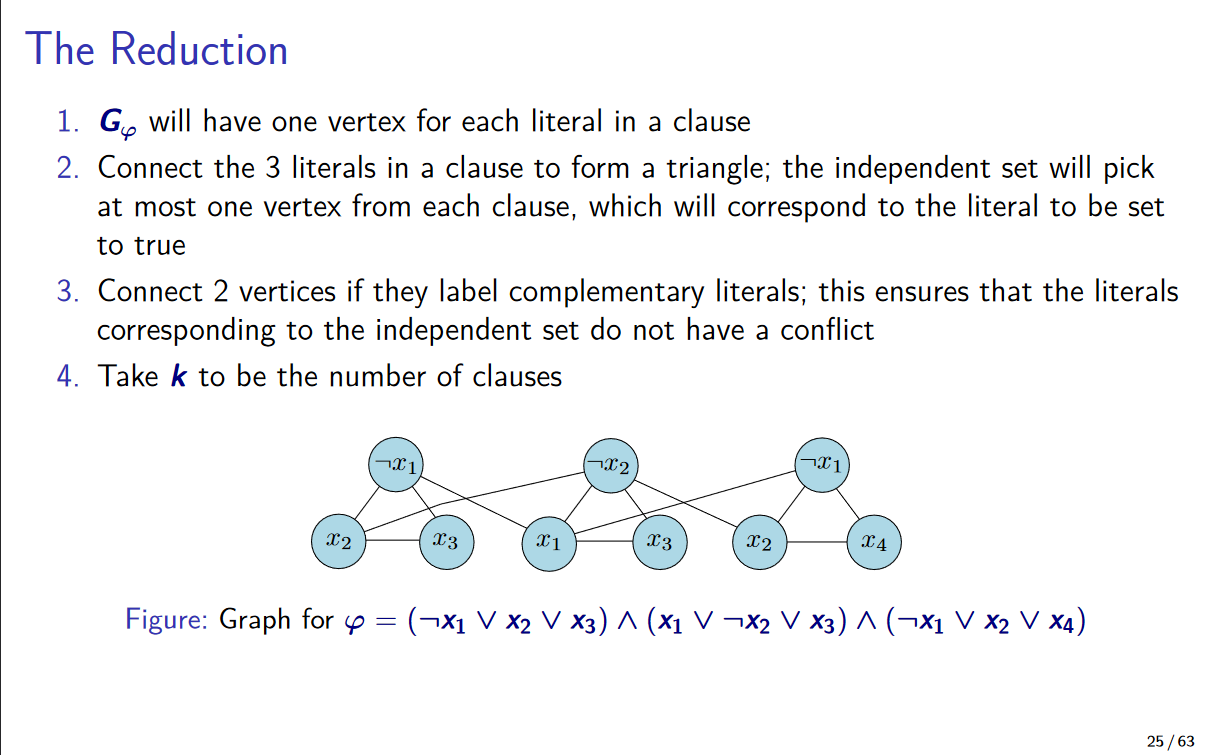
\includegraphics[width=\textwidth]{NI-KOP/tutorials/files/05-sat-to-is}
\end{figure}

\vspace{4pt}
\noindent Vidíme, že zde půjde každý krok převést v polynomiálním čase. Platí ale naše ekvivalence? Pokud je formule splnitelná, pak platí v každé klauzuli min. 1 literál a díky konstrukci vím, že za každou klauzuli bude v cílové množině \textbf{právě jeden} uzel, budou tedy 3. Tak stejně obrácený směr: z konstrukce vidíme, že to bude opravdu splnitelné. \href{https://courses.engr.illinois.edu/cs374/fa2020/lec_prerec/23/23_2_0_0.pdf}{Podrobný důkaz zde.}

\subsection{Problém 3--SAT}

Jak budeme konstruovat Karpovu \textbf{redukci}? Vstupem bude SAT formule a výstupem bude 3--SAT formule. Potřebuji vyřešit správně počet literálů na vstupu.

\vspace{4pt}
\noindent Když mám tři literály, je to ok. Když jsou dva $(b+c)$, převedu to na $(b+c+x), (b+c+\lnot{}x)$. Když je jeden, přidám tam $x_1, x_2$ ve 4 variantách. Když jich je více: např. 4 -- rozdělím na $(a+b+x_1), (c+d+x_2)$. \href{https://cse.iitkgp.ac.in/~palash/2018AlgoDesignAnalysis/SAT-3SAT.pdf}{Náčrt důkazu zde.}

\begin{figure}[H]
\centering
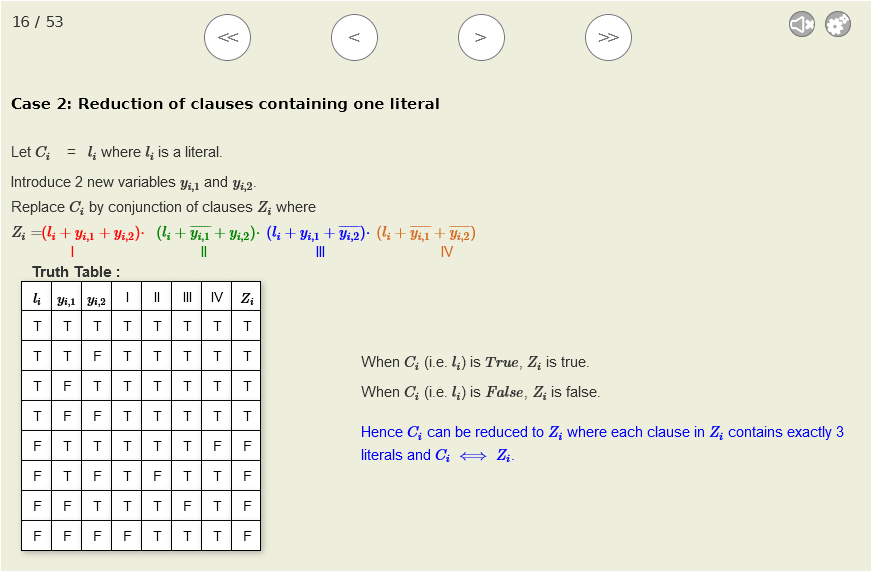
\includegraphics[width=0.8\textwidth]{NI-KOP/tutorials/files/05-sat-to-3sat}
\end{figure}

\section{Stavový prostor}

Co jsou\textbf{ konfigurační proměnné} u SATu? Co je jeho certifikát? Jsou to \textbf{ohodnocení} $Y$ jednotlivých proměnných $x_1, \ldots, x_n$, tedy funkce $y_1 = Y(x_1), \ldots$

\vspace{4pt}
\noindent Co je \textbf{stavový prostor} algoritmu A řešícího instanci I problému $\Pi$? Je to \textbf{uspořádaná dvojice} stavů a operátorů, které umožňují přechod mezi nimi. U SATu jsou stavy \textbf{ohodnocení} jednotlivých \textbf{konfiguračních proměnných} ($x_m$) a operátory budou \textbf{funkce}, které dané proměnné změní stav (např. $Y(x_m)$ = $\lnot x_m$).

\vspace{4pt}
\noindent Tento graf u GSATu je \textbf{silně souvislý}, bude vypadat jako n-rozměrná krychle, mezi jednotlivými stavy se přesunu v $m$ krocích, kde $m$ je Hammingova vzd.

\vspace{4pt}
\noindent Už známe hledání typu BFS, DBS, nebo podle prioritní fronty \textit{(prioritou je hodnota optimalizačního kritéria)}. To je \textbf{systematické} prohledávání, nebo dokonce \textbf{úplné}.

\vspace{4pt}
\noindent Existují ale způsoby, které prostě můžou skončit v nějakém \blockquote{lokálním minimu} -- best only, first improvement\ldots

\vspace{4pt}
\noindent Hra \textbf{sokoban}: stavem nejsou polohy beden, ale sekvence pohybů beden.
